\documentclass{article}

% Language setting
% Replace `english' with e.g. `spanish' to change the document language
\usepackage[english]{babel}

% Set page size and margins
% Replace `letterpaper' with `a4paper' for UK/EU standard size
\usepackage[letterpaper,top=2cm,bottom=2cm,left=3cm,right=3cm,marginparwidth=1.75cm]{geometry}

% Useful packages
\usepackage{amsmath}
\usepackage{graphicx}
\usepackage[colorlinks=true, allcolors=blue]{hyperref}

\title{Exposé Intelligent Agents Geomates Practicals}
\author{Ali Baran Oez, Mohammad Ghassan Aburas, Martin Stuwe, Jendrik Stoltz}

\begin{document}
\maketitle

\section{Main Idea}

The main Idea of our agent is the combination of planning systems and a Large Language Model on different levels of control of the agent. 
With the capability of LLMs of handling loosely defined tasks, the LLM gets tasked to find subgoals / critical points in the level and select one of them as the first goal. As communication is hard with unknown agents in the level,  the Theory of Mind capabilities of LLMs discussed in the lecture are expected to select actions that fit to what the other agent might do in the situation. 

Planning Systems on the other hand offer deterministic results and do not have the hallucination problem of LLMs in complex reasoning tasks ensuring correct plans for reaching goals. Planning systems also have a lower answer latency and are much lighter on resources. 

In our System the LLM therefore only selects subgoals (Lifted Planning) and a PDDL Planner finds a sequence of atomic actions that lead to the subgoal (Grounded Planning). A success or Fail of the plan as well as critical changes in the world affecting the goal are reported to the LLM to react / choose the next subgoal.

\section{Self Localisation}

The self localisation of the agent gets handled by a startup routine that gets executed before giving control to the actual agent code. To find out if the ball or the rectangle are controlled, a "W" command gets send to the game after a wait period derived from the PID of the process. If the ball position changes on the y axis, the agent controls the ball, if the shape of the rectangle changes the agent controls the rectangle. If both changes are observed, the process gets repeated after a random wait interval. When the agent type is determined, control is given to the agent logic.

\section{Agent Structure}

In \ref{fig:architecture} an overview of our agent structure is given. The Agent interacts with the world through a world connector that handles Telnet communication with the game. It takes WASD contol from the Low Level Controller and provides the current world description to the modules of the agent. The Low Level Controller executes a plan of atomar actions the agent can do. Each atomar action consists of a PID controller callback for executing the action, an action description for the PDDL planner containing preconditions and effects as well as state flags indicating a success or fail. The low level controller also checks if something in the world affects a future part of the plan (e.g. other agent in the way, goal diamond gone, atomar action failed) and stops plan execution then. Success and fail of a plan are reported to the LLM with the current world state to find a new subgoal based on the new state.
\begin{figure}[h]
\caption{Architectural Overview}
\label{fig:architecture}
\centering
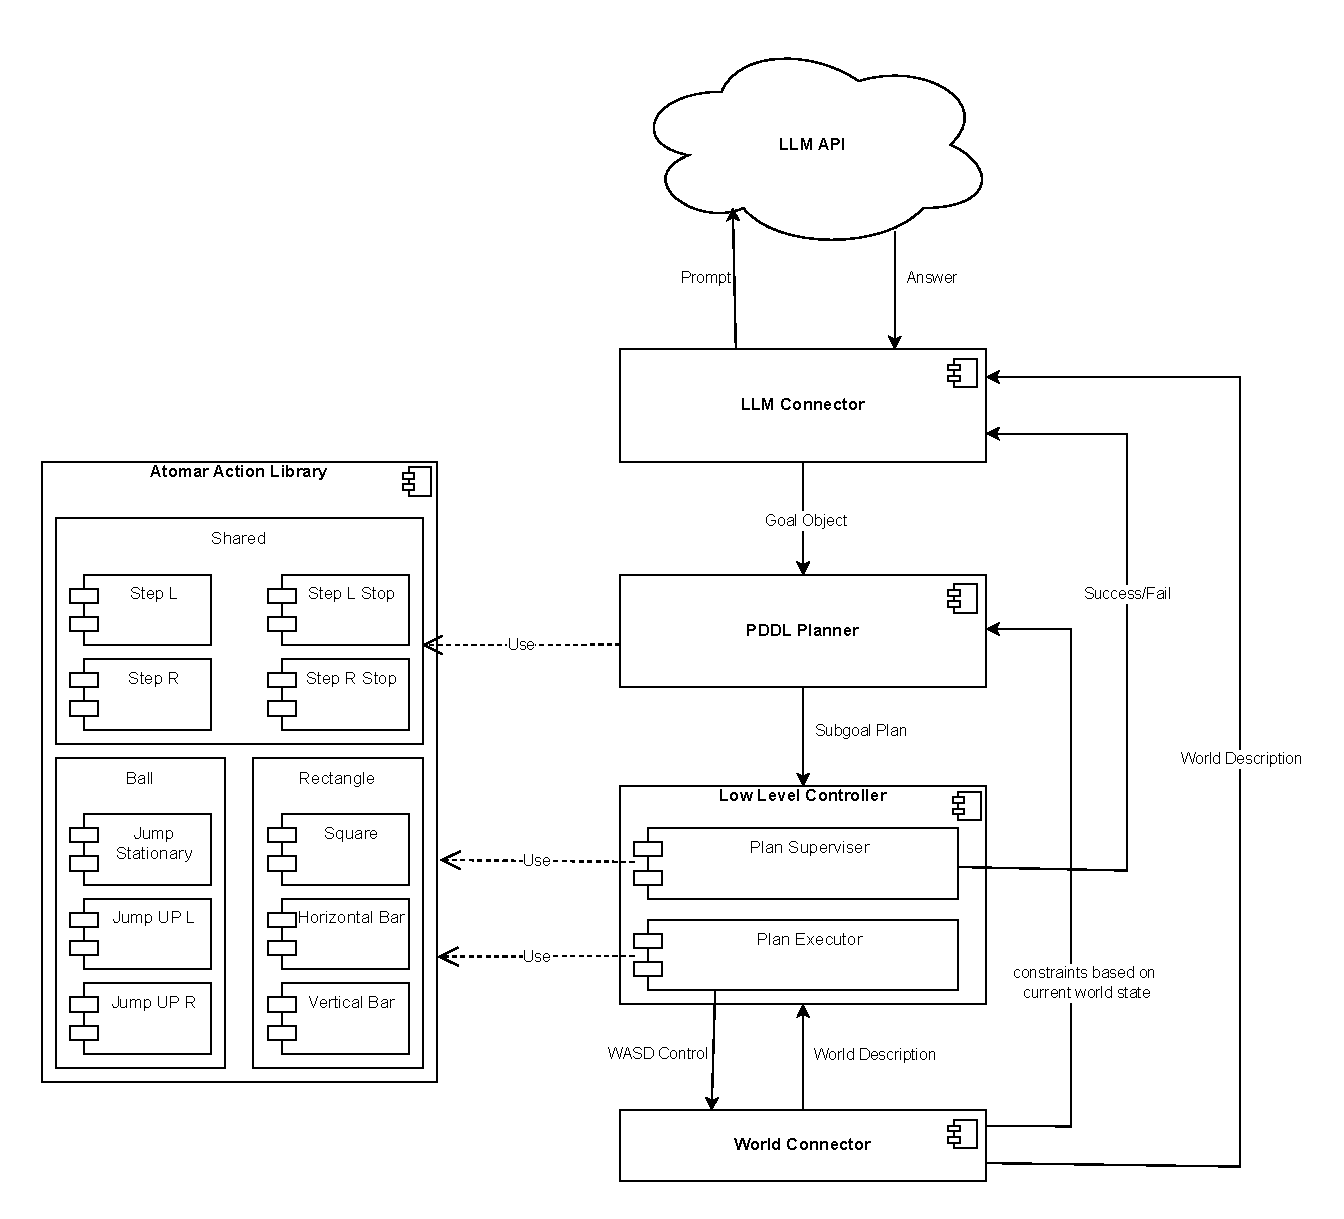
\includegraphics[width=0.7\textwidth]{graphic/IA_llm_agent.pdf}
\end{figure}

\section{Learning through LLM in-context learning}

Requests to the LLM for planning the next tasks are accompanied by a history of actions and their effect. This information can therefore be used to adapt to past behavior of the other agent and success of plans. If the history gets not resetted between levels we hope that the LLM gets better at developing a theory of mind of the other agent and get a better "feeling" of the viability of goals.

\section{Collaboration}

On its own, our agent will only select diamonds as goals and do not offer cooperation. The other player will however be considered in Planning and will be reported to the LLM. If the position of another agent gets considered useful for collecting a goal it can get used. For future development however specific predefined helpful situations could be identified and be proposed to the LLM

\section{Agent Evaluation}

We plan to evaluate our agent in levels containing 
We expect our agent to perform particularly well in levels where It is important to collect diamonds that are not targeted by the other agent like diamonds that are hard to reach and far away for the controlled player but easy to reach and close for the other player. Also cooperation with an agent that offers help (simulated by manual control) could work well. We see problems in Levels containing traps and unrecoverable states as the LLM may have problems understanding the game physics.

\section{Organization}

The Project can be split up in different work packets that can be worked on individually.

\subsection{Software Architecture}
To make the different components of the system work together, a software architecture and a framework defining the structure and communication of the application and the different components has to be defined. 
The logic and behaviour of the different components will then be added in this framework. 
The goal of this work package is a working python framework with callbacks for communication between the modules and defined interfaces. 
It will also include Communication with the simulation via the World connector. The person responsible for this task is Jendrik Stoltz. 
As integration of the other functionality depends on this task, it has to be worked on early on.

\subsection{Self Localisation}
To find out which object our model controls, a "W" command is sent to the game, from the world definition we can detect the change in the Y-axis for the circle or the change in the height for the rectangle. Depending on the change, we can evaluate which object is controlled by our agent. To do this, first, the initial positions and dimensions of the rectangle and circle objects are determined and after waiting for a while after the command, it can be checked whether there is a change. If there is no change for either object after the command, the "A" or "D" command can be sent and the change in the X-axis can be checked. This can be useful in cases where there is a movement restriction at the beginning in some sections. The reason why the "W" command was used instead of the "A" or "D" command at the beginning was chosen to prevent objects from falling by considering that they can spawn on a platform in certain levels. At this point, considering that the other model may also start to localize itself with a similar method, it may be appropriate to choose a more distinctive movement combination. For this reason, by sending the "W" command 3 times in a row, the number of Y position changes for the circle or the number of length changes for the rectangle can be followed.

\subsection{Low Level Control}
The goal of this work package is the creation of a library of atomic actions for the square and rectangle with the required P(I)D controllers. It will also include a plan executor that will run an action sequence and check for success or fail.
A draft of preconditions and effects of the atomic actions for later use in the planner is also included. The person responsible for this task is Jendrik Stoltz.

\subsection{Connect Planner to World and Actions}
% Martin, Mohammad

The goal of this work package is to ensure that the high-level planning module (PDDL planner) is effectively connected to the actual actions executed in the game world. This integration is crucial for translating abstract subgoals into concrete, atomic actions performed by the agent. The connection is implemented through the following process:

\begin{enumerate}
    \item \textbf{Plan Generation:}  
    Once the LLM selects a subgoal, the PDDL planner is invoked to generate a sequence of atomic actions that lead toward that subgoal. Each atomic action is defined with:
    \begin{itemize}
        \item A description containing its \emph{preconditions} and \emph{effects}.
        \item A corresponding callback function that invokes a PID controller to execute the movement or operation.
    \end{itemize}
    
    \item \textbf{Action Execution:}  
    The generated plan is handed off to the Low-Level Controller, which sequentially executes each atomic action. The controller uses the world connector to send commands (via Telnet) to the game environment.
    
    \item \textbf{World State Monitoring:}  
    Throughout execution, the world connector continuously receives updated world state information. This monitoring enables the system to verify if:
    \begin{itemize}
        \item The preconditions for the next action are still met.
        \item The executed action produced the intended effects.
        \item External events (e.g., interference from the other agent, disappearance of critical objects) necessitate plan revision.
    \end{itemize}
    
    \item \textbf{Feedback and Re-planning:}  
    If an atomic action fails or if the current world state invalidates the plan (for instance, due to unexpected interference), the Low-Level Controller interrupts the ongoing plan execution. A detailed report, including the failure mode and current world context, is sent back to the LLM. The LLM can then use this feedback to choose a new subgoal, and the planning process starts anew.
    
    \item \textbf{Error Handling and Robustness:}  
    Robust error-handling mechanisms are in place to address discrepancies between the expected and actual world states. This includes:
    \begin{itemize}
        \item Logging all atomic action outcomes.
        \item Dynamically adjusting action parameters via PID controllers.
        \item Initiating recovery procedures when critical failures are detected.
    \end{itemize}
\end{enumerate}

This tight integration of planning, execution, and feedback ensures that the deterministic strengths of the PDDL planner are leveraged while still allowing real-time adjustments based on dynamic game conditions.

\subsection{LLM Setup and Prompt Design}
% Martin, Mohammad

Since the agent runs on hardware with limited GPU resources, we rely on a remote API for the LLM. The chosen provider (e.g., Google Gemini) is expected to meet our usage constraints—less than 15 requests per minute (RPM), fewer than 1 million tokens per minute (TPM), and under 1,500 requests per day (RPD).

\textbf{API Setup:}
\begin{itemize}
    \item \textbf{Provider Selection:}  
    The LLM is accessed through a remote API, ensuring that our agent can perform advanced reasoning without requiring local GPU resources.
    
    \item \textbf{Connection and Authentication:}  
    Secure connections are established to the API endpoint, with proper authentication protocols in place. Rate limiting and error-handling procedures are also implemented to handle potential network issues or API downtimes.
    
    \item \textbf{Scalability Considerations:}  
    Given our relatively low usage expectations, the API configuration is optimized to maintain low latency while ensuring that each prompt-response cycle is efficient.
\end{itemize}

\textbf{Prompt Design:}
\begin{itemize}
    \item \textbf{Compact World Representation:}  
    The prompt is designed to provide the LLM with a concise yet informative snapshot of the current game state. This includes:
    \begin{itemize}
        \item The agent’s current position and status.
        \item The state and location of nearby objects (e.g., diamonds, traps).
        \item Observations regarding the other agent’s behavior.
        \item A summary of the recent action history and outcomes.
    \end{itemize}
    
    \item \textbf{Clear Instruction for Subgoal Selection:}  
    The prompt explicitly instructs the LLM to analyze the current state and propose a new subgoal. The instruction emphasizes criteria such as avoiding conflict with the other agent and selecting a subgoal that is viable given the current environmental conditions.
    
    \item \textbf{Dynamic Context Injection:}  
    A prompt template is used, wherein placeholders are dynamically populated with the latest world state and history data before sending the request. This helps the LLM leverage its in-context learning capabilities and develop a rudimentary theory of mind regarding the other agent.
    
    \item \textbf{Token Efficiency:}  
    To meet API limitations and ensure fast response times, the prompt is optimized to include only essential details.
\end{itemize}

A sample prompt template might look like this:

\begin{verbatim}
[World State]
- Agent Position: (x, y)
- Nearby Objects: [list with positions and statuses]
- Other Agent Observations: [brief summary of movements/actions]
- Recent Action History: [actions and outcomes]

Task: Based on the above state, determine the next viable subgoal that advances our overall objective while minimizing interference with the other agent.
\end{verbatim}

Once the prompt is sent to the LLM, the response is parsed to extract the recommended subgoal. This subgoal is then forwarded to the PDDL planner for generating the corresponding sequence of atomic actions, thereby closing the loop between high-level reasoning and low-level execution.

By combining a robust, remote LLM setup with a carefully designed prompt, our system leverages the flexible reasoning capabilities of the LLM while maintaining deterministic control through grounded planning.



\subsection{Evaluation}
Ali

\subsection{Deployment}
The Goal of this work package is the creation of the final deliverable, a fully working docker container containing the agent. 
This task will be tackled by the group when the agent is working as a standalone application.


\end{document}
